\section{Methods}\label{sec:method}
The goal is to adapt a pretrained VLA to complete language-conditioned manipulation tasks on a target robot. We study multi-stage pick-and-place tasks: an instruction such as \emph{put the apple on the plate} requires approach, grasp, lift, transport, and release. The policy receives camera images, proprioception, and an instruction, predicts an action chunk, and executes a prefix before observing again. We evaluate complete-task success independently of the reward used for training.

During acquisition, each skill has its own instruction, success condition, and starting states. For example, placement can begin with an object already held. During composition and final evaluation, the robot starts with an empty gripper and receives one complete-task instruction. This distinction prevents isolated skill performance from being treated as full-task success.


\subsection{Dense Acquisition, Binary Refinement, and Self-Imitation}\label{sec:skill_acquisition}
We use dense rewards only at the beginning of adaptation to learn a base policy for simple skills. Each skill has a distinct instruction and reset distribution:
\begin{itemize}
\item \textbf{Approach:} \emph{move to \textless object\textgreater}. Reach the named object with an empty gripper, without requiring a grasp.
\item \textbf{Pickup:} \emph{pick up \textless object\textgreater}. Learn to grasp and lift the named object.
\item \textbf{Placement:} \emph{put \textless object\textgreater\ into bowl} or \emph{put \textless object\textgreater\ on the plate}. Start with the object already grasped and learn transport and release at the named destination.
\end{itemize}
The object placeholder is replaced by its name. These instructions condition the policy on the requested skill and target; the instruction remains attached to each retained trajectory. Distance reduction and manipulation events guide initial acquisition. We then refine the skills with binary success rewards and consolidate them through self-imitation. The resulting base policy must retain all component skills before full-task learning.

Successful trajectories are retained by instruction. When later training degrades earlier skills, self-imitation fits a balanced mixture of earlier and current successes:
\begin{equation}
\mathcal L_{\rm SI}=\mathbb E_{\rm success}
\left[\|\hat a-a\|^2\right].
\label{eq:si_loss}
\end{equation}
Here $\hat a$ is the predicted action and $a$ is the recorded executed action. The average balances instructions and excludes unused action slots. Policy-dependent features are refreshed before fitting. Balancing matters because imitating only the newest skill can reinforce forgetting.

Algorithm~\ref{alg:paper_pipeline} summarizes the schedule. Progress is checked with fixed skill evaluations. After an initial training period, automated stages can end at a success target or a plateau; budget exhaustion also ends a stage. The CDPR sequence used validation-guided manual transitions. After consolidation, all learned skills are evaluated again. Automated runs retain the consolidation update only when recovery improves the degraded skills on average and keeps other skills within tolerance.
% Method-level schedule. Automatic stopping is implemented for WX200;
% the historical CDPR sequence used validation-guided manual transitions.
\begin{algorithm}[!t]
\caption{Staged VLA adaptation}
\label{alg:paper_pipeline}
\small
\begin{algorithmic}[1]
\Require Pretrained VLA, simple-skill instructions, fixed evaluations
\State Initialize the target action controller and success banks
\For{reward mode: dense acquisition, then binary refinement}
    \For{skill: approach, pickup, placement}
        \Repeat
            \State Collect same-scene rollout groups for the skill
            \State Update with $\mathcal L_{\rm RL}$; retain successful trajectories
            \State Evaluate skill success
        \Until{target, plateau, or stage budget ends training}
        \State Evaluate retention of all learned skills
        \If{earlier skills have degraded}
            \State Balance earlier and current successful experience
            \State Fit $\mathcal L_{\rm SI}$; validate recovery and retention
        \EndIf
    \EndFor
\EndFor
\State Initialize full-task learning from the consolidated base policy
\Repeat
    \State Collect full-task rollouts from empty-gripper starts
    \State Assign milestone credit; protect achieved prefix skills
    \State Update with $\mathcal L_{\rm RL}$; evaluate complete-task success
\Until{target, plateau, or full-task budget ends training}
\If{composition plateaus and budget remains}
    \State Freeze VLA/LoRA; retain the bounded residual
    \State Reset optimizer; keep milestone rewards unchanged
    \Repeat
        \State Collect full-task groups; execute clipped commands
        \State Store pre-clipping samples and episode offsets
        \State Score samples conditional on their stored offsets
        \State Assign milestone credit; protect achieved prefix skills
        \State Update residual and exploration with $\mathcal L_{\rm RL}$
        \State Evaluate complete-task success
    \Until{target, renewed plateau, or budget exhaustion}
\EndIf
\State \Return One policy for the complete instruction
\end{algorithmic}
\end{algorithm}


\subsection{SmolVLA with an Embodiment-Specific Residual}
\begin{figure*}[!t]
\centering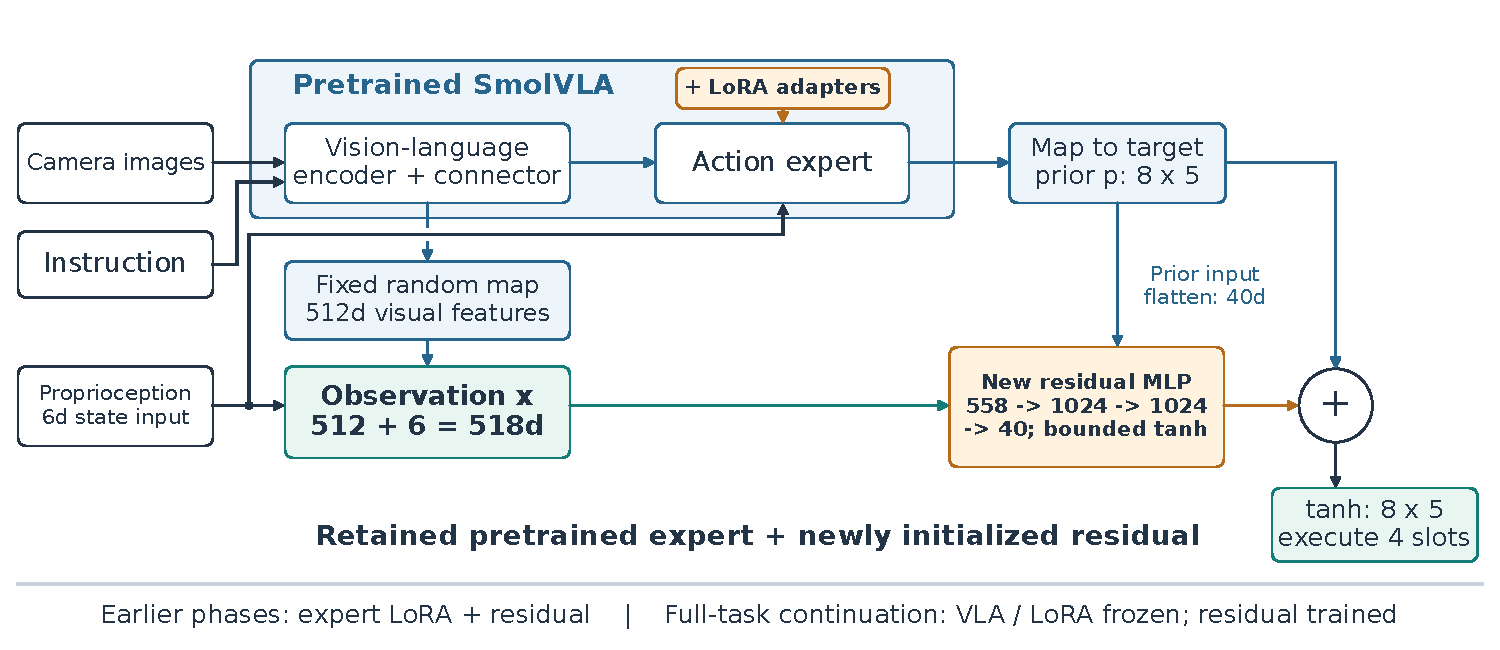
\includegraphics[width=\textwidth]{figures/smolvla_residual_lora.pdf}
\caption{SmolVLA implementation of the pipeline. The added residual combines 518 observation features with a 40-dimensional action prior. LoRA adapts the pretrained expert during earlier training; the evaluated full-task continuation freezes the VLA and LoRA weights. Feature and action dimensions refer to the five-channel controller.}
\label{fig:architecture}
\end{figure*}

Figure~\ref{fig:architecture} shows one implementation of the pipeline. Following the residual-learning ingredient of Probe, Learn, Distill (PLD)~\cite{pld}, we retain a pretrained expert and adapt its actions with a lightweight residual. The SmolVLA expert supplies an action prior, mapped to the target control interface. In our five-channel controller, eight action slots form a 40-dimensional prior.
A frozen visual projection supplies 512 features; six proprioceptive values complete the 518-dimensional observation. The residual receives this observation and the 40-dimensional prior, and predicts a bounded correction. The combined action is bounded before execution.

LoRA adapts the action expert during earlier training. In the evaluated full-task continuation, the inherited VLA and LoRA weights are frozen while the residual and exploration parameters are trained. The backbone, action mapping, and feature dimensions can change with the embodiment; the training schedule remains the same.


\subsection{Milestone-Based Full-Task Composition}\label{sec:composition}
After skill consolidation, the base policy learns the complete task from empty-gripper starts using binary milestone rewards. The full-task prompt is \emph{put \textless object\textgreater\ into \textless destination\textgreater}, where the destination is plate or bowl. This includes the plate wording \emph{into plate}, whereas the isolated plate-placement skill uses \emph{on the plate}. The full-task instruction stays fixed throughout approach, pickup, and placement. Each milestone marks completion of part of this sequence. Continuous dense shaping is confined to the initial simple-skill acquisition in Section~\ref{sec:skill_acquisition}. The LIBERO reward comparison examines how intermediate feedback can support execution of a complete instruction.

\label{sec:dense_method}
We consider terminal-only, phase-only, and combined dense-and-phase rewards. The combined reward uses a manually defined sequence of reach, grasp, lift, move, and place phases, with a hand-specified progress function for each phase.

At each simulator step, the tracker uses object and gripper state to compute progress for the active phase. Reaching progress increases as gripper--object distance decreases; grasping combines proximity with gripper closure and grasp state; lifting uses height gained above the initial object position; transport uses planar object--target distance; placement uses target proximity, release, and environment success. Each progress measure is normalized to the interval from zero to one. For progress $p_t$ and the phase's previous maximum $p_{\rm best}$, the rewarded increment is $\max(p_t-p_{\rm best},0)$. A completion predicate advances the tracker to the next phase and produces a phase bonus. The weighted progress increment and phase bonus are bounded and combined with terminal feedback. The native task-success verifier remains unchanged.

In the phase-only condition, the continuous progress weight is zero, leaving phase-completion bonuses and terminal feedback.

The dense construction requires a progress function, normalization, and relevant state variables for every phase. Extending it to a new multi-stage task therefore requires further task-specific reward design. Our adaptation pipeline uses this detailed feedback only to obtain the initial base policy on simple skills. Full-task training uses binary milestones and their completion predicates, so the composition stage does not require a continuous progress function for every part of the instruction.

The motivation follows from a simple group calculation. For $G$ independent rollouts from one scene, each with success probability $p$, the probability of observing both success and failure is
\begin{equation}
P_{\rm mixed}=1-p^G-(1-p)^G.
\label{eq:mixed}
\end{equation}
With eight rollouts, this probability is only 21.6\% at 3\% success, but 94.2\% at 30\% success. Milestones can therefore provide informative comparisons before complete-task success becomes common.


In the adapted CDPR controller, approach, held pickup, and final placement serve as milestones for assigning credit within a rollout. The policy executes the complete instruction without an external controller switching between specialists.

The main rule is simple: a later placement failure should not remove the local credit for a successful approach or pickup. We compare milestone outcomes within groups of rollouts from the same scene. Actions receive credit for the milestone they contribute to, while full-task success provides an additional preference for completing the chain. A negative completion bonus is suppressed on already achieved approach and pickup milestones. Placement receives its completion credit once.

The rule retains the assigned credit for completed milestones while training the remaining task.

\subsection{Stabilized Updates and Full-Task Continuation}\label{sec:rl_loss}
We use a clipped group-relative policy loss with entropy regularization:
\begin{equation}
\mathcal L_{\rm RL}=\mathcal L_{\rm clip}-\eta\mathcal H.
\label{eq:rl_loss}
\end{equation}
The clipped loss compares rollouts within each scene group and limits the incentive for large changes in action likelihood. We use separate upper and lower clipping bounds. The entropy term $\mathcal H$, weighted by $\eta$, maintains exploration during manipulation and composition. Together, these choices help keep early updates conservative while successful behavior is still rare.

During skill learning, DAPO-style dynamic sampling filters uninformative groups and collects additional rollout groups within the configured collection budget~\cite{dapo}. With binary rewards, uniform outcomes provide no group-relative contrast. During dense acquisition, filtering instead checks within-group return variation, so partial progress can provide a learning signal before a group contains a successful skill execution.

During full-task continuation, the inherited VLA and LoRA remain frozen while the residual and exploration scale are trained with a fresh optimizer and the same milestone rewards. The controller adds Gaussian exploration noise and an episode-level offset to its predicted mean before clipping the command for execution. The offset is sampled once per episode and applied during selected phases. We store the original sample and the applied offset, then use both to evaluate its likelihood under the old and new policies~\cite{capg}.

Let $\mu_{\theta,t}$ denote the controller's predicted mean, $\sigma_\theta$ the learned exploration scale, and $b_t$ the applied offset. The sampled command $u_t$ and executed action $a_t$ are
\begin{equation}
\begin{aligned}
u_t&\sim\mathcal N(\mu_{\theta,t}+b_t,\operatorname{diag}(\sigma_\theta^2)),\\
a_t&=\operatorname{clip}(u_t,-1,1).
\end{aligned}
\label{eq:latent_action}
\end{equation}
The likelihood ratio scores the stored $u_t$ conditional on the same $b_t$. Section~\ref{sec:cdpr_results} reports complete-task performance.
